
\chapter{Turbulence in the Arctic}
\label{john:turbulence}

\begin{center}								% center the text horizontally

\textit{John Lennon \& Paul McCartney}				% names of all authors

\vspace{1cm}

\begin{minipage}{0.9\textwidth}				% minipage with a width of 0.9 times the total text width, just a matter of personal taste
\centerline{\textbf{\large Abstract}}
\vspace{0.3cm}
\lipsum[1]									% abstract text

\end{minipage}
\end{center}

\vspace{1cm}

\section{Introduction}		% the next smaller level after chapter is section...
\label{john:introduction}
\lipsum[1] \citep{nilsen2016simple}.		% latex style to cite a paper from your .bib file. two ways: \citet{•} puts the brackets only around the year, e.g. "I've read it in Einstein et al., (1915)." \citep{•} puts the brackets around everything, like you did it most of the times..., see https://www.overleaf.com/learn/latex/natbib_citation_styles

\begin{figure}[htbp]		% typical way to include a figure. The option [htbp] means, that the compiler should try to place it Here first (that's why h first), then at the Top of the next page (t as second letter), at the bottom of the page (b) and as last option wherever it fits best...
    \centering				% center the figure horizontally
    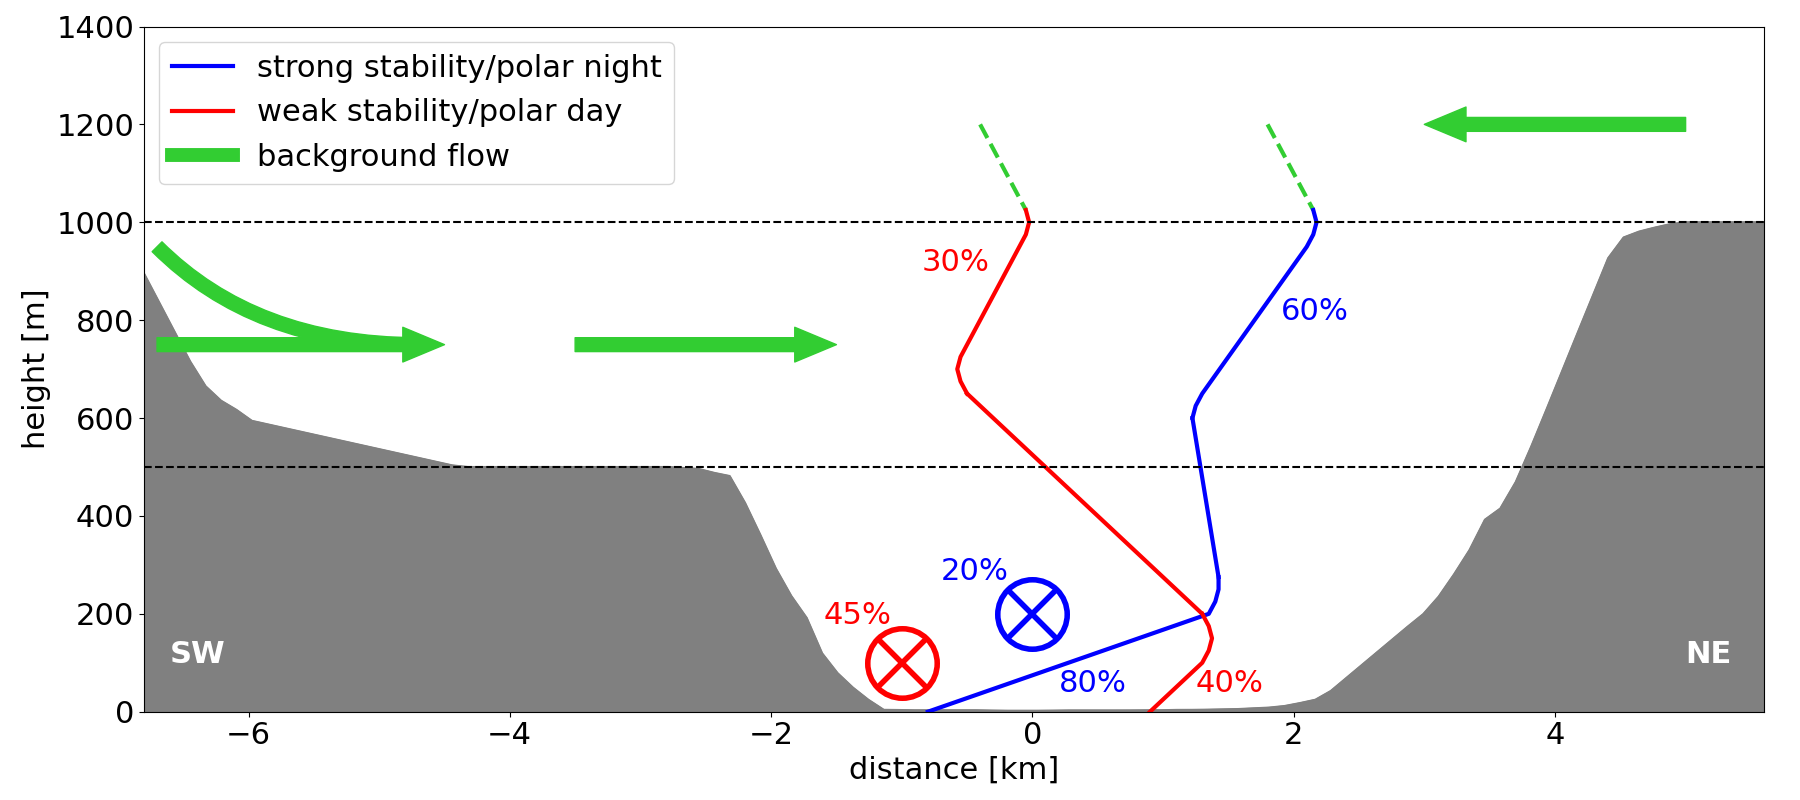
\includegraphics[width=\textwidth]{./figures_john/schematic_ABL.png}
    \vspace{-20pt}		% put the caption a little closer to the figure
    \caption[Short description for list of figures]{Longer description to be printed under the figure, can include references like \citep{stull1988introduction}} % The text in the curly brackets is what appears below the figure, the text in the square brackets appears in the list of figures. In that way, you can give it a shorter description for the list and a longer text to put actually with the figure.
	\label{john:fig1}		% label to reference to the figure in the text (I've learned, that you need to refer to every figure in your document at least once... You should doublecheck that with your supervisor)
\end{figure}

\lipsum



\section{Theory}
\label{john:theory}
\subsection{Turbulent fluxes}
\label{john:fluxes}
\lipsum


\section{Data \& Methods}
\label{john:methods}
\lipsum

\section{Results}
\label{john:results}
\lipsum

% example for a table:
\begin{table}[htbp]
    \setlength\belowcaptionskip{1.5ex}
    \centering
    \caption[Stability regime definitions]{Definitions and total occurrence frequencies (during Period One) of the stability regime used within this study.}
    \label{john:table_stab_regimes}
    \begin{tabular}{|c|c|c|c|}
    \hline
    \textbf{Regime} & \textbf{Abbreviation} & \textbf{range of MOST} & \textbf{occurrence frequency/} \\
     & & \textbf{stability parameter} & \textbf{total data points} \\ \hline
    unstable & us & $\zeta < 0.0$ & 27.09\,\% / 11\,808 \\ \hline
    nearly neutral & nn & $0.0 \leq \zeta < 0.02$ & 15.78\,\% / 6\,878 \\ \hline
    weakly stable & ws & $0.02 \leq \zeta < 0.7$ & 52.25\,\% / 22\,776 \\ \hline
    very stable & vs & $0.7 \leq \zeta < 3.0$ & 4.20\,\% / 1\,833 \\ \hline
    extremely stable & es & $\zeta \geq 3.0$ & 0.69\,\% / 299 \\ \hline
    \end{tabular}
\end{table}

Reference to Table \ref{john:table_stab_regimes} looks like this ...


\section{Discussion}
\label{john:discussion}
\lipsum

\section{Conclusions \& Outlook}
\label{john:conclusion}
\lipsum

\vspace{3cm}
% lists for figures, tables, literature...
\bibliography{biblio_john}
\bibliographystyle{apalike}